% Spacious paper-style overview of the complete MSA--OCV--GBC MixerCSeg.
% The encoder and decoder are separated vertically to keep all routes legible.
\newcommand{\overallfeature}[7]{%
  \begin{scope}[shift={(#2,#3)}]
    \foreach \k in {3,2,1,0}{
      \draw[draw=#4!72!black, fill=#4!20, line width=0.45pt]
        ({-#5/2+0.075*\k},{-#6/2+0.075*\k}) rectangle
        ({ #5/2+0.075*\k},{ #6/2+0.075*\k});
    }
  \end{scope}
  \node[minimum width=#5cm, minimum height=#6cm, inner sep=0pt] (#1) at (#2,#3) {};
  \node[font=\sffamily\scriptsize, align=center, anchor=north]
    at ($(#1.south)+(0,-0.16)$) {#7};
}

\begin{tikzpicture}[
  font=\sffamily\footnotesize,
  >=Latex,
  flow/.style={->, very thick, draw=black!72},
  featureflow/.style={->, thick, draw=blue!64!black},
  attention/.style={->, thick, draw=orange!82!black},
  region/.style={draw, rounded corners=3pt, line width=0.65pt},
  stage/.style={draw=cyan!65!black, fill=cyan!10, rounded corners=2pt,
    text width=16mm, minimum width=18mm, minimum height=17mm,
    align=center, inner sep=1.5pt, font=\sffamily\scriptsize},
  pm/.style={draw=gray!60, fill=gray!10, rounded corners=1.5pt,
    minimum width=8mm, minimum height=9mm, align=center, inner sep=1pt,
    font=\sffamily\scriptsize},
  block/.style={draw=blue!52!black, fill=blue!6, rounded corners=2pt,
    minimum height=11mm, align=center, inner sep=2.2pt},
  fuse/.style={draw=purple!55!black, fill=purple!7, rounded corners=2pt,
    minimum height=12mm, align=center, inner sep=2.2pt},
  head/.style={draw=orange!75!black, fill=orange!16, rounded corners=2pt,
    minimum width=10mm, minimum height=18mm, align=center, inner sep=2pt},
  op/.style={draw=black!65, circle, fill=white, minimum size=5.8mm,
    inner sep=0.4pt, font=\sffamily\scriptsize\bfseries},
  title/.style={font=\sffamily\small\bfseries, anchor=west}
]

% ------------------------------------------------------------------
% Input and four-stage encoder.
% ------------------------------------------------------------------
\filldraw[region, fill=gray!1, draw=gray!22] (0,0) rectangle (20.2,10.55);
\node[title] at (0.28,10.23) {Overall architecture of MSA--OCV--GBC MixerCSeg};

\begin{scope}[yshift=0.8cm]
\node[draw=black!50, fill=white, inner sep=1.2pt] (input) at (0.92,6.82)
  {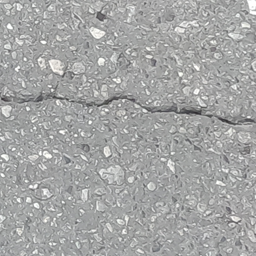
\includegraphics[width=1.42cm]{../dataset/CrackMap/test_img/GOPR0317 (5).png}};
\node[font=\sffamily\scriptsize, below=1.0mm of input] {CrackMap input};
\node[draw=orange!70!black, fill=orange!12, rounded corners=2pt,
  minimum width=9mm, minimum height=20mm, align=center] (stem) at (2.35,6.82)
  {Stem\\$3\!\rightarrow\!16$\\$128^2$};
\draw[flow] (input) -- (stem);

\filldraw[region, fill=cyan!3, draw=cyan!30] (3.02,4.22) rectangle (13.30,8.75);
\node[font=\sffamily\footnotesize\bfseries, anchor=west] at (3.28,8.45)
  {Four-stage encoder};

\node[stage] (s1) at (4.05,6.88) {Stage 1\\TransMixer\\+ GAB};
\node[pm]    (pm1) at (5.42,6.88) {PM\\$\downarrow2$};
\node[stage] (s2) at (6.80,6.88) {Stage 2\\TransMixer\\+ GAB};
\node[pm]    (pm2) at (8.17,6.88) {PM\\$\downarrow2$};
\node[stage] (s3) at (9.55,6.88) {Stage 3\\TransMixer\\+ GAB};
\node[pm]    (pm3) at (10.92,6.88) {PM\\$\downarrow2$};
\node[stage] (s4) at (12.30,6.88) {Stage 4\\TransMixer\\+ GAB};

\draw[flow] (stem) -- (s1);
\draw[flow] (s1) -- (pm1);
\draw[flow] (pm1) -- (s2);
\draw[flow] (s2) -- (pm2);
\draw[flow] (pm2) -- (s3);
\draw[flow] (s3) -- (pm3);
\draw[flow] (pm3) -- (s4);

\overallfeature{f1}{4.05}{5.08}{cyan}{0.62}{0.72}{$F_1$\\$16\!\times\!128^2$}
\overallfeature{f2}{6.80}{5.08}{blue}{0.58}{0.66}{$F_2$\\$32\!\times\!64^2$}
\overallfeature{f3}{9.55}{5.08}{blue}{0.54}{0.60}{$F_3$\\$64\!\times\!32^2$}
\overallfeature{f4}{12.30}{5.08}{violet}{0.50}{0.55}{$F_4$\\$128\!\times\!16^2$}
\draw[featureflow] (s1.south) -- (f1.north);
\draw[featureflow] (s2.south) -- (f2.north);
\draw[featureflow] (s3.south) -- (f3.north);
\draw[featureflow] (s4.south) -- (f4.north);
\end{scope}

% ------------------------------------------------------------------
% SRF decoder.  Four vertical projection routes stay separated.
% ------------------------------------------------------------------
\filldraw[region, fill=blue!2, draw=blue!26] (3.02,0.05) rectangle (16.00,4.65);
\node[font=\sffamily\footnotesize\bfseries, anchor=east] at (15.72,4.35)
  {SRF decoder};

\node[block, minimum width=18mm] (p1) at (4.05,3.45) {$F_1$ projection\\$16\!\rightarrow\!8$};
\node[block, minimum width=18mm] (p2) at (6.80,3.45) {$F_2$ projection\\$32\!\rightarrow\!8$};
\node[block, minimum width=18mm] (p3) at (9.55,3.45) {$F_3$ projection\\$64\!\rightarrow\!8$};
\node[block, minimum width=18mm] (p4) at (12.30,3.45) {$F_4$ projection\\$128\!\rightarrow\!8$};

\draw[featureflow] (f1.south) -- (p1.north);
\draw[featureflow] (f2.south) -- (p2.north);
\draw[featureflow] (f3.south) -- (p3.north);
\draw[featureflow] (f4.south) -- (p4.north);

\node[block, minimum width=19mm] (att) at (4.05,0.85) {$1{\times}1$ Conv\\$A=\sigma(\cdot)$};
\draw[attention] (p1) -- (att);

\node[block, minimum width=17mm] (up1) at (5.05,2.08) {$F_1$ upsample\\to $512^2$};
\draw[featureflow] (p1.south) -- ++(0,-0.16) -| (up1.north);

\node[block, minimum width=23mm] (align) at (9.55,0.85)
  {Align $F_{2:4}$\\to $128\!\times\!128$};
\draw[featureflow] (p2.south) -- ++(0,-0.48);
\draw[featureflow] (p3.south) -- ++(0,-0.48);
\draw[featureflow] (p4.south) -- ++(0,-0.48);
\draw[featureflow, -] ($(p2.south)+(0,-0.48)$) -- ($(p4.south)+(0,-0.48)$);
\draw[featureflow] ($(p3.south)+(0,-0.48)$) -- (align.north);

\node[op] (mul) at (11.25,0.85) {$\odot$};
\draw[featureflow] (align) -- (mul);
\draw[attention] (att.south) -- ++(0,-0.14) -| (mul.south);

\node[block, minimum width=17mm] (up234) at (12.53,0.85) {Upsample\\to $512^2$};
\draw[featureflow] (mul) -- (up234);

\node[fuse, minimum width=10mm, minimum height=17mm] (cat) at (13.85,1.72)
  {Concat\\32 ch};
\node[fuse, minimum width=11mm, minimum height=17mm] (fusion) at (15.22,1.72)
  {Conv/GN\\$32\!\rightarrow\!8$};
\draw[featureflow] (up1.east) -- ++(0.30,0) -| (cat.north);
\draw[featureflow] (up234.east) -| (cat.south);
\draw[flow] (cat) -- (fusion);

% ------------------------------------------------------------------
% Prediction head and a real output probability map.
% ------------------------------------------------------------------
\node[head] (seg) at (16.78,1.72) {Prediction\\head};
\node[draw=black!50, fill=white, inner sep=1.2pt] (output) at (18.62,1.72)
  {\includegraphics[width=1.42cm]{../results/probability_maps/triple_stack_v4_crackmap/validate_v3_msa_ocv_gbc_seed42/GOPR0317 (5)_pre.png}};
\node[font=\sffamily\scriptsize, below=1.0mm of output] {Predicted crack map};
\draw[flow] (fusion) -- (seg);
\draw[flow] (seg) -- (output);

\end{tikzpicture}
